\documentclass[10pt,a4paper]{article}
\usepackage[utf8]{inputenc}
\usepackage{amsmath}
\usepackage{amsfonts}
\usepackage{amssymb}
\usepackage{graphicx}
\usepackage{enumerate}
\begin{document}

\section{Set Theory}

To demystify mathematics consider
\begin{enumerate}[(i)]
\item What is a theorem?
\item What is a proof?
\end{enumerate}
What if we don't know the answer?

To begin we need
\begin{enumerate}[(a)]
\item an example(s)
\item a nearly related concept
\end{enumerate}


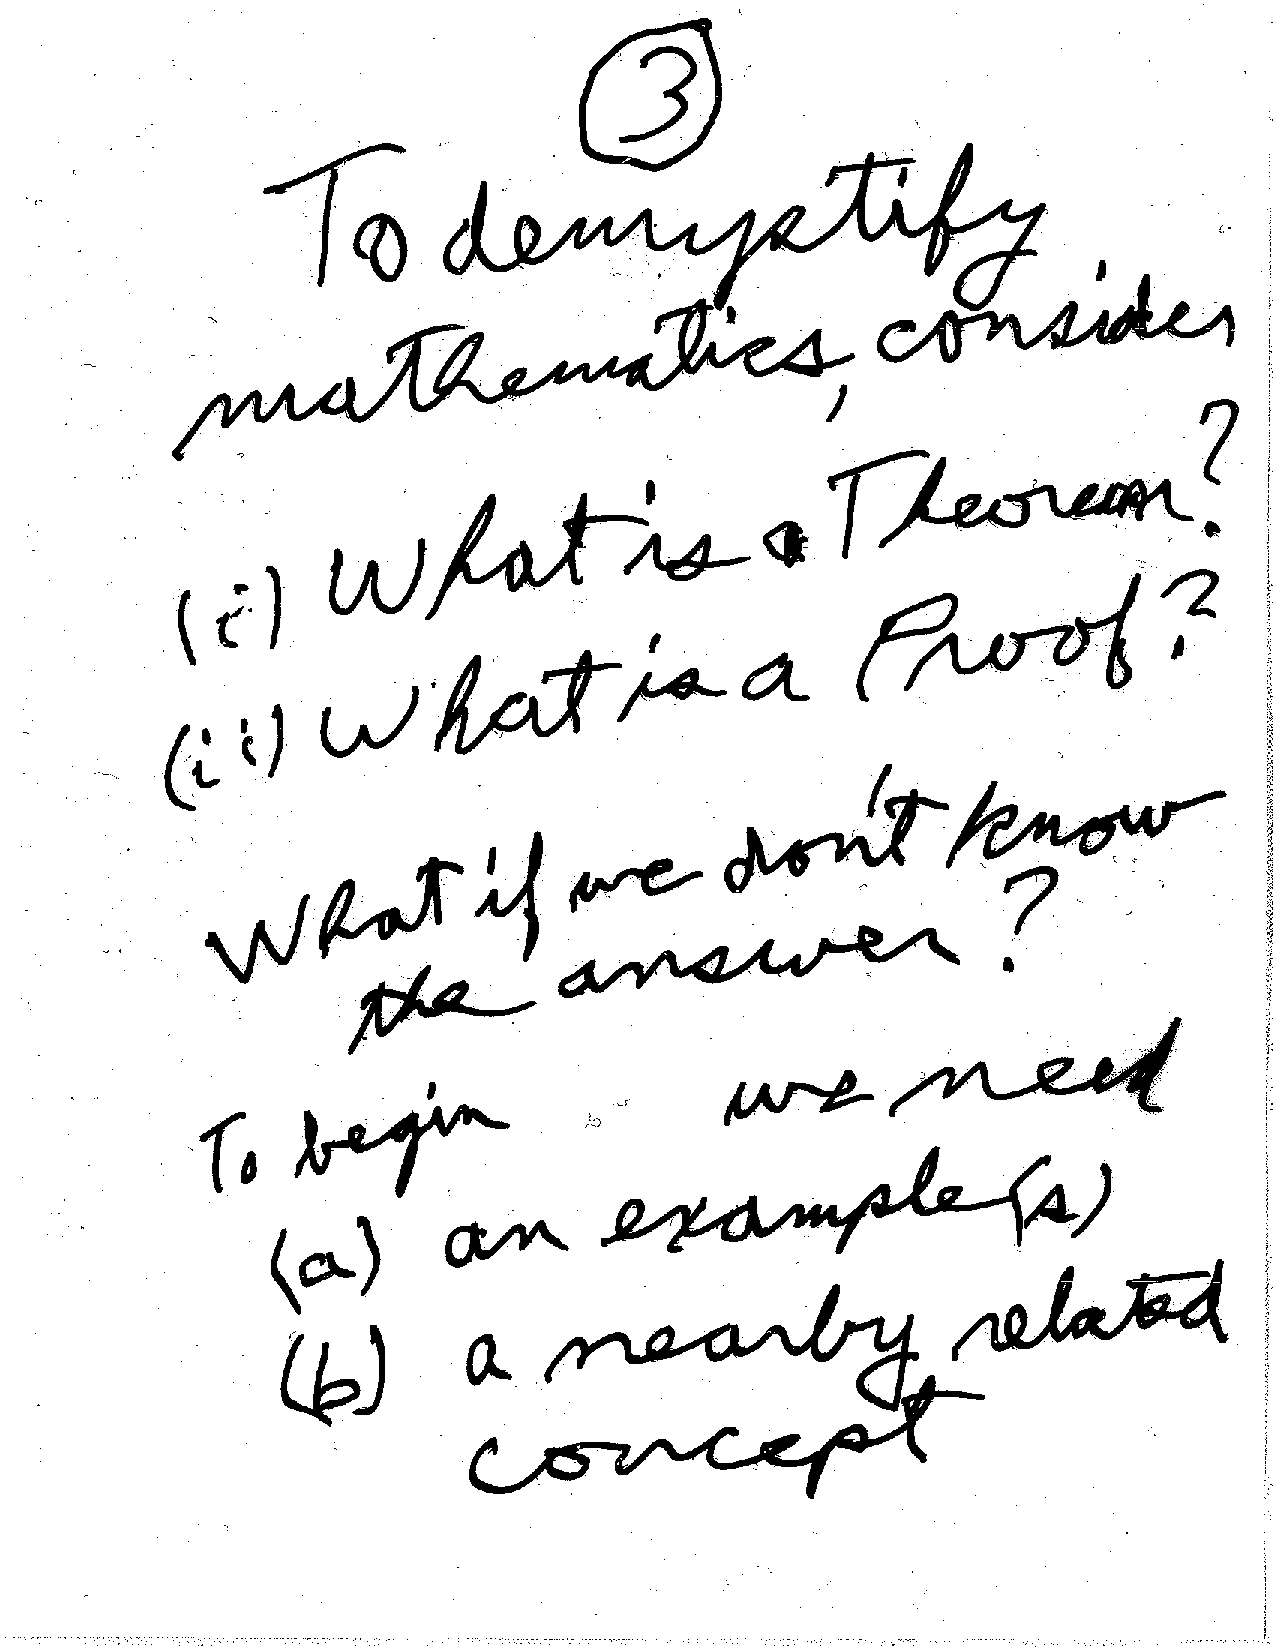
\includegraphics[scale=.5]{Pages/ST_3}

\newpage

Related Concept: Greek Syllogism

\underline{example:}
\begin{enumerate}
\item All men are mortal.
\item Socrates is a man.
\item Therefore, Socrates must die. 
\end{enumerate}

To analyze, recast in set theoretic terms via Venn Diagram.

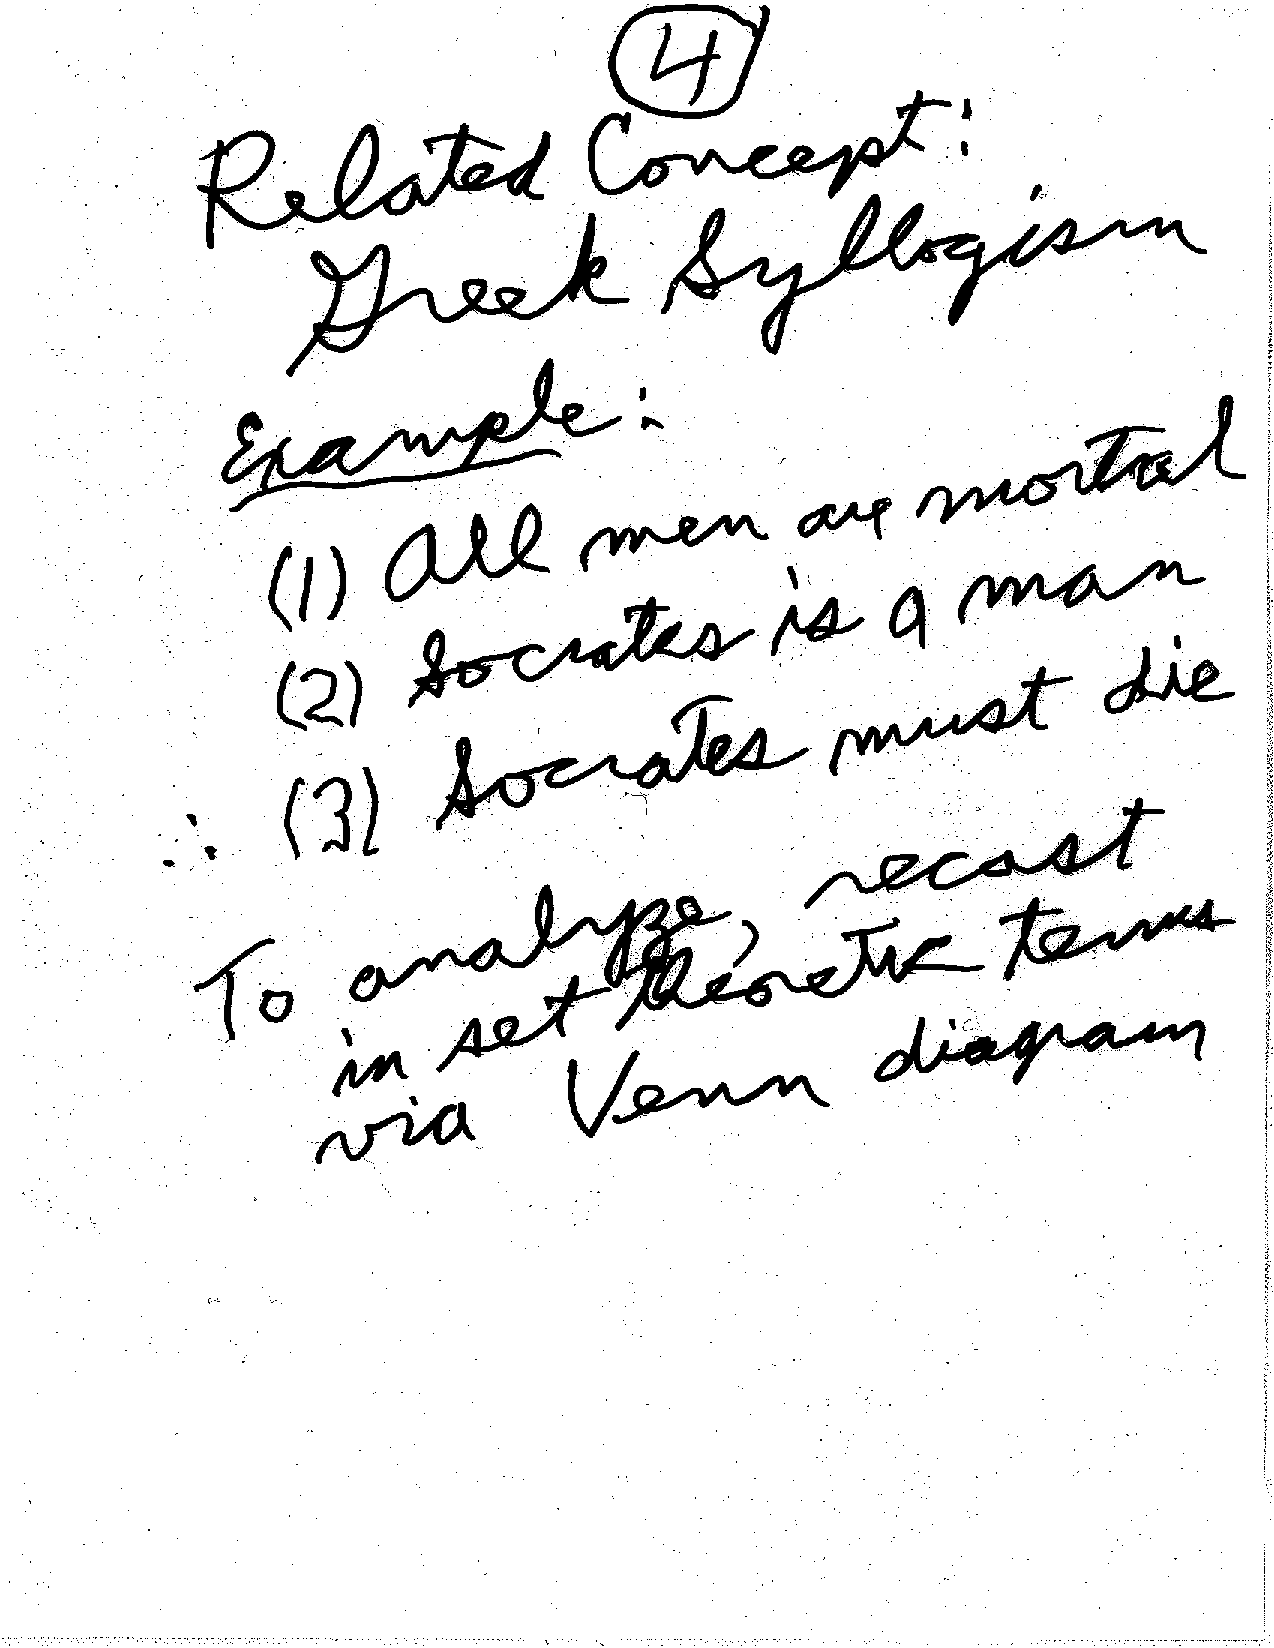
\includegraphics[scale=.5]{Pages/ST_4}

\newpage

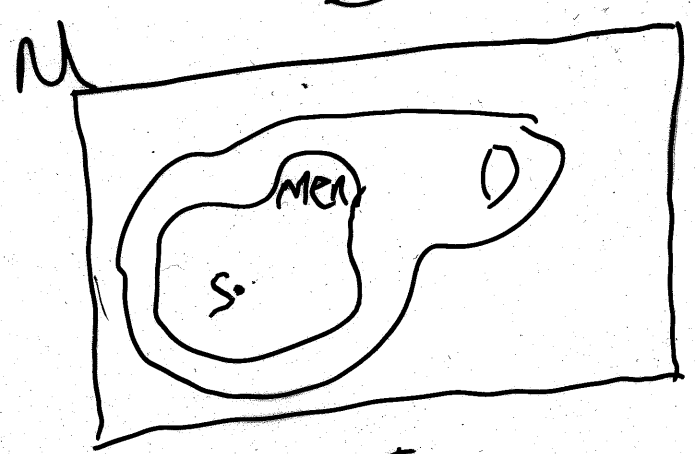
\includegraphics[scale=.2]{Pages/ST_5_im1}

$S$: Socrates\\
$M$: Set of Men\\
$D$: Things that will die\\
$\mathcal{U}$: Things on Earth

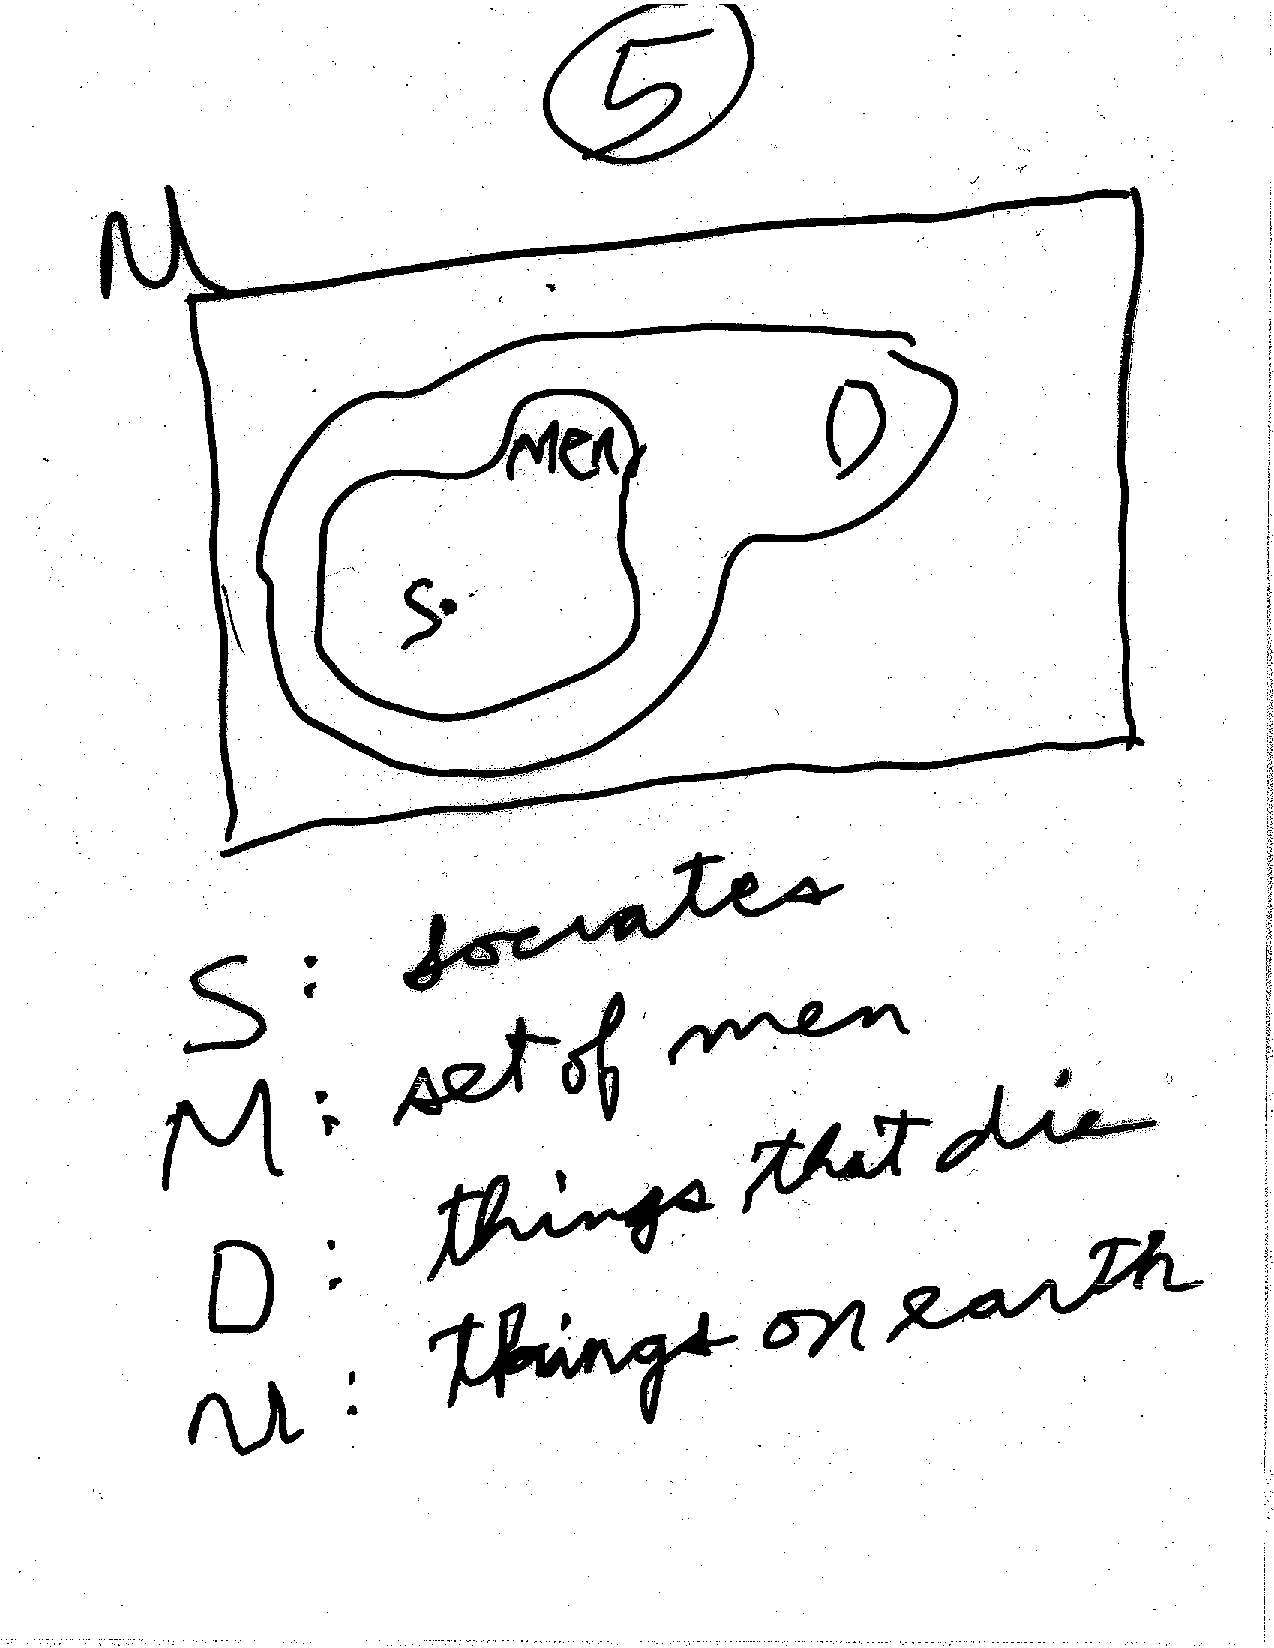
\includegraphics[scale=.5]{Pages/ST_5} 



%Zack: Pages 6,7,8,19,20

%Jack: 21, 9, 10, 11

%Koka: Pages 13, 13A, 22 ,22A, 22B


\section{Generate $\mathbb{N}$}


%Ruth: Pages L4A-L4G




\section{From $\mathbb{Z}$ to $\mathbb{R}$ via ordering}
%Jazz: ZR1-ZR5

%Kyler: ZR6 - ZR10

%Preethika: ZR11-ZR14


\section{Sequence and Limits}

%Aaron: First 2 pages and 48-50

Sequences

Limits

Constructing the limit via:

\begin{enumerate} [(i)]

\item Monotonic Sequences
\item Monotonic Sub-sequences 

\end{enumerate}

Cauchy Sequences

Subsequential Limits 

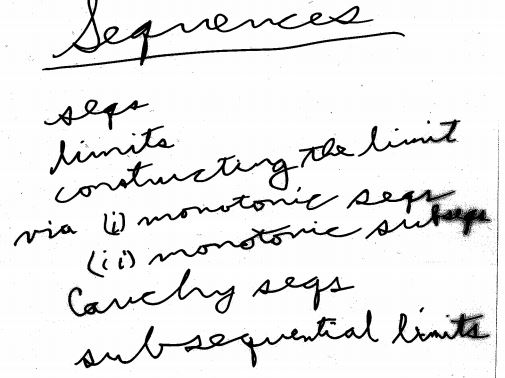
\includegraphics[scale=.8]{Pages/S&L_page1}

\newpage


Besides $\vec{a}$ = $(a{_0}, a_{1}, a_{2}, ...)$, how else might we harness elements of $\mathbb {R}^{2}$?

$$s_0 = a_{0}$$

$$s_1 = a_{0} + \frac{a_{1}}{2}$$



$$s_{n} = \sum_{j=0}^{n} a_{j} 2^{-j}$$




The sequence $\{s_{n}\}$ represents \{ ${z \in \mathbb{Z}_{\infty} : z < s_{n}} $ for all in sufficient large \}

It has a limit of $s_{\infty}$

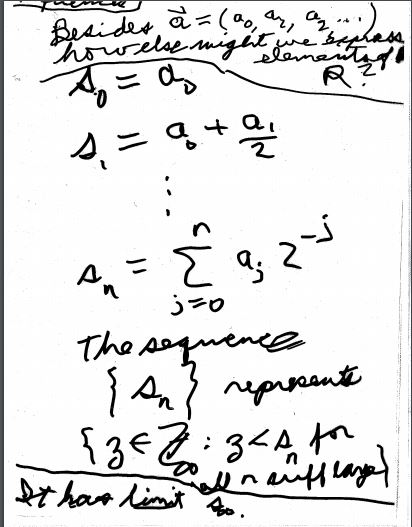
\includegraphics[scale=.8]{Pages/S&L_page2}

\newpage
{\bf Sequences}


Def: a sequence \{ ${a_n}_{1}^\infty$ \} is a map from the integers. A real valued sequence is a map into the reale from the integers.

Examples:

\begin{enumerate} [{}]

\item $a{_n}$ = $\frac{1}{n^{2}}$
\item $a_{n} = (-c)^{n}$
\item $a_{n} = \cos(nx)$
\item $a_{n} = n^\frac{1}{n}$
\item $a_{n} = (1 + \frac{1}{n})^{n}$

\end{enumerate}

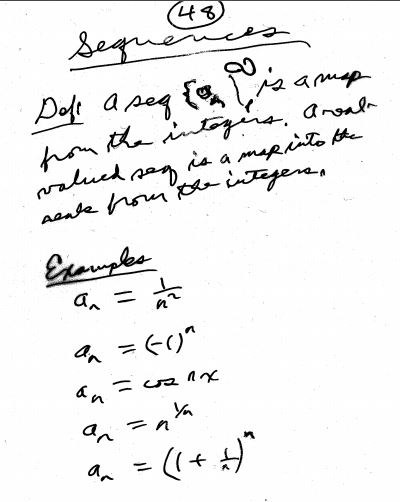
\includegraphics[scale=.8]{Pages/S&L_page48}

\newpage

{\bf Convergence of Sequences} 

Def: $a_{n} \rightarrow a$ if and only if $\forall \epsilon > 0\exists N$:

for all n $\geq N$, $|a_{n} - a| < \epsilon$

we write... $$a = \lim_{n \rightarrow \infty} a_{n}$$

Def: $a_{n} \rightarrow + \infty$ if and only if $\forall b < \infty$ $\epsilon N_{b}$ such that for all $n \geq , N_{b} , a_{n} \geq b$ 

Def: $a_{n} \rightarrow - \infty$ ?

Then (limits are unique)

if $a_{n} \rightarrow a$ and $a_{n} \rightarrow b$

then $a=b$

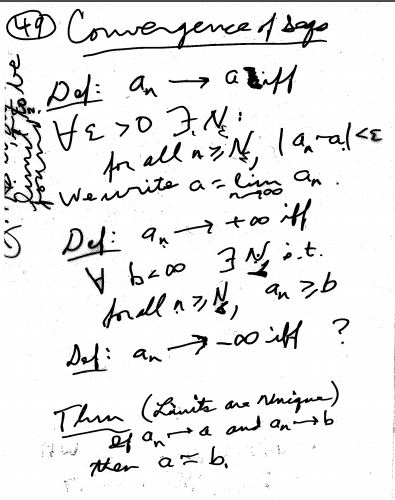
\includegraphics[scale=.8]{Pages/S&L_page49(1)}

\newpage

{\bf Convergence in $\mathbb {R}_{\infty}$ An Elegant Reformation}

Def: Let $\{ a_{n} \}$ be a sequence of reals and $a_{\infty} \epsilon \mathbb {R} \bigcup$ $\{  \pm \infty \}$ .

$\lim_{n \rightarrow \infty} a_{n} = a_{\infty}$ if and only if...

\begin{enumerate} [(i)]

\item $\forall$ real $b > a_{\infty}$

$\exists N_{b} < \infty$ : for all

$n \geq N_{b}$, $a_{n} < b$

\end{enumerate}

and

\begin{enumerate} [(ii)]

\item $\forall$ real $b < a_{\infty}$

$\exists N_{b} < \infty$: for all

$n \geq N_{b}$, $a_{n} > b$

\end{enumerate}

you prove

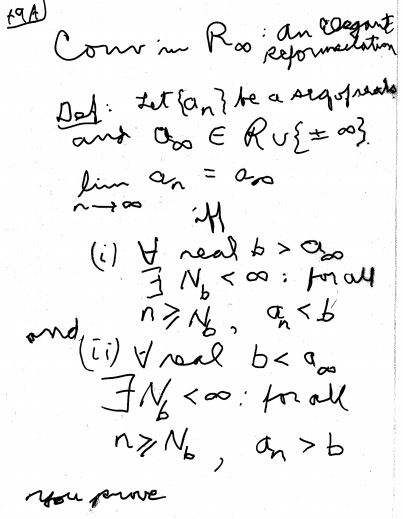
\includegraphics[scale=.7]{Pages/S&L_page49(2)}

\newpage


{\bf Finding Limits and Proving Convergence}

Example 1: $\lim_{n \rightarrow \infty} \frac{1}{n^{2}} = 0$

Example 2: $\lim_{n \rightarrow \infty} \frac{3n+1}{7n-4} = \frac{3}{7}$

Example 3: $\lim_{n \rightarrow \infty} (1 + \frac{1}{n})^{n} = e$

Homework: Suppose $a_{n} \rightarrow a > 0$


Prove $\sqrt{a_{n}} \rightarrow \sqrt{a}$

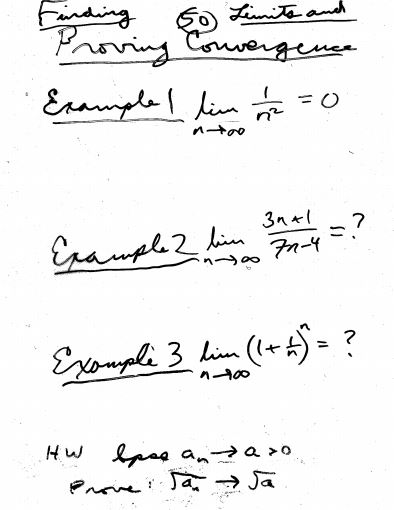
\includegraphics[scale=.7]{Pages/S&L_page50}

\newpage











%Hamza: 51-52B

\section{Limit and Convergence}

%Joe: 50-51

%Quinten: 52-53

%Farishta: 53A-54A

\section{Infinite Series}

%Sukhreet: IS1 - IS 7

%Matthew: IS8 - IS15

%Will: IS16 - IS23

%Rebecca: IS24 - IS32

%Maady: IS33 - IS42

\section{Metric Spaces Part 1}

%Travis: M1 - M5

%Jerome: M6- M10



\section{Metric Spaces Part 2}


%Bryant: M1-M7

%Reshma: M8-M14

%Ethan: M15-M21





\end{document}